\renewcommand{\one}{fake_022}
\renewcommand{\two}{fake_039}

\setlength{\resLen}{.45in}
\begin{figure}[t]
	\addtolength{\tabcolsep}{-4pt}
	\begin{tabular}{ccccc}
		& \textbf{\footnotesize{SVBRDF maps}} & \textbf{\small Opt.} & \multicolumn{2}{c}{\textbf{\small Novel views}}
		\\
		\raisebox{.2in}{\rotatebox[origin=c]{90}{\footnotesize{GT}}} &
		\includegraphics[height=\resLen]{results/fake/\one/ref/tex.jpg} &
		\includegraphics[height=\resLen]{results/fake/\one/ref/00.jpg} &
		\includegraphics[height=\resLen]{results/fake/\one/ref/07.jpg} &
		\includegraphics[height=\resLen]{results/fake/\one/ref/08.jpg}
		\\
		\raisebox{.2in}{\rotatebox[origin=c]{90}{\footnotesize{Ours}}} &
		\includegraphics[height=\resLen]{results/fake/\one/ours+/tex.jpg} &
		\includegraphics[height=\resLen]{results/fake/\one/ours+/00.jpg} &
		\includegraphics[height=\resLen]{results/fake/\one/ours+/07.jpg} &
		\includegraphics[height=\resLen]{results/fake/\one/ours+/08.jpg}
		\\
		\raisebox{.2in}{\rotatebox[origin=c]{90}{\footnotesize{GT}}} &
		\includegraphics[height=\resLen]{results/fake/\two/ref/tex.jpg} &
		\includegraphics[height=\resLen]{results/fake/\two/ref/00.jpg} &
		\includegraphics[height=\resLen]{results/fake/\two/ref/07.jpg} &
		\includegraphics[height=\resLen]{results/fake/\two/ref/08.jpg}
		\\
		\raisebox{.2in}{\rotatebox[origin=c]{90}{\footnotesize{Ours}}} &
		\includegraphics[height=\resLen]{results/fake/\two/ours+/tex.jpg} &
		\includegraphics[height=\resLen]{results/fake/\two/ours+/00.jpg} &
		\includegraphics[height=\resLen]{results/fake/\two/ours+/07.jpg} &
		\includegraphics[height=\resLen]{results/fake/\two/ours+/08.jpg}
	\end{tabular}
	\caption{\label{fig:synthetic}
		\textbf{SVBRDF reconstruction on synthetic data.} We demonstrate results on synthetic SVBRDFs, one from \cite{Deschaintre2019} (top) and one from the Adobe Stock Material dataset (bottom). We are able to accurately reconstruct these materials from 7 input images (one input shown). Many more synthetic results are available in supplementary materials.
	}
\end{figure}